%%%%%%%%%%%%%%%%%%%%%%%%%%%%%%%%%%%%%%%%%
% Short Sectioned Assignment LaTeX Template Version 1.0 (5/5/12)
% This template has been downloaded from: http://www.LaTeXTemplates.com
% Original author:  Frits Wenneker (http://www.howtotex.com)
% License: CC BY-NC-SA 3.0 (http://creativecommons.org/licenses/by-nc-sa/3.0/)
%%%%%%%%%%%%%%%%%%%%%%%%%%%%%%%%%%%%%%%%%

%----------------------------------------------------------------------------------------
%	PACKAGES AND OTHER DOCUMENT CONFIGURATIONS
%----------------------------------------------------------------------------------------

\documentclass[paper=a4, fontsize=11pt]{scrartcl} % A4 paper and 11pt font size

% ---- Entrada y salida de texto -----

\usepackage[T1]{fontenc} % Use 8-bit encoding that has 256 glyphs
\usepackage[utf8]{inputenc}

% ---- Idioma --------

\usepackage[spanish, es-tabla]{babel} % Selecciona el español para palabras introducidas automáticamente, p.ej. "septiembre" en la fecha y especifica que se use la palabra Tabla en vez de Cuadro

% ---- Otros paquetes ----

\usepackage{amsmath,amsfonts,amsthm} % Math packages
\usepackage{graphics,graphicx, floatrow} %para incluir imágenes y notas en las imágenes
\usepackage{graphics,graphicx, float} %para incluir imágenes y colocarlas
\usepackage{hyperref} % url in references
\usepackage{textcomp}
\usepackage{listings}
\usepackage{titlesec}

% Para hacer tablas comlejas
\usepackage{multirow}
\usepackage{threeparttable}

\usepackage{fancyhdr} % Custom headers and footers
\pagestyle{fancyplain} % Makes all pages in the document conform to the custom headers and footers
\fancyhead{} % No page header - if you want one, create it in the same way as the footers below
\fancyfoot[L]{} % Empty left footer
\fancyfoot[C]{} % Empty center footer
\fancyfoot[R]{\thepage} % Page numbering for right footer
\renewcommand{\headrulewidth}{0pt} % Remove header underlines
\renewcommand{\footrulewidth}{0pt} % Remove footer underlines
\setlength{\headheight}{13.6pt} % Customize the height of the header

\numberwithin{equation}{section} % Number equations within sections (i.e. 1.1, 1.2, 2.1, 2.2 instead of 1, 2, 3, 4)
\numberwithin{figure}{section} % Number figures within sections (i.e. 1.1, 1.2, 2.1, 2.2 instead of 1, 2, 3, 4)
\numberwithin{table}{section} % Number tables within sections (i.e. 1.1, 1.2, 2.1, 2.2 instead of 1, 2, 3, 4)

\setlength\parindent{0pt} % Removes all indentation from paragraphs - comment this line for an assignment with lots of text

\newcommand{\horrule}[1]{\rule{\linewidth}{#1}} % Create horizontal rule command with 1 argument of height


%----------------------------------------------------------------------------------------
%	DATOS
%----------------------------------------------------------------------------------------

\newcommand{\myName}{Francisco Javier Bolívar Lupiáñez}
\newcommand{\myDegree}{Grado en Ingeniería Informática}
\newcommand{\myFaculty}{E. T. S. de Ingenierías Informática y de Telecomunicación}
\newcommand{\myDepartment}{Lenguajes y Sistemas de Información}
\newcommand{\myUniversity}{\protect{Universidad de Granada}}
\newcommand{\myLocation}{Granada}
\newcommand{\myTime}{\today}
\newcommand{\myTitle}{Práctica 1}
\newcommand{\mySubtitle}{Implementación distribuida de un algoritmo paralelo de datos usando MPI}
\newcommand{\mySubject}{Programación Paralela}
\newcommand{\myYear}{2015-2016}

%----------------------------------------------------------------------------------------
%	PORTADA
%----------------------------------------------------------------------------------------


\title{	
	\normalfont \normalsize 
	\textsc{{\bf \mySubject \space (\myYear)} \\ \myDepartment} \\[20pt] % Your university, school and/or department name(s)
	\textsc{\myDegree \\[10pt] \myFaculty \\ \myUniversity} \\[25pt]
	\horrule{0.5pt} \\[0.4cm] % Thin top horizontal rule
	\huge \myTitle: \mySubtitle \\ % The assignment title
	\horrule{2pt} \\[0.5cm] % Thick bottom horizontal rule
	\normalfont \normalsize
}

\author{\myName} % Nombre y apellidos

\date{\myTime} % Incluye la fecha actual
%----------------------------------------------------------------------------------------
%	INDICE
%----------------------------------------------------------------------------------------

\begin{document}

\lstdefinestyle{C} {
	basicstyle=\scriptsize,
	frame=single,
	language=C,
	numbers=left
}

\titleformat{\paragraph}{\sffamily\bfseries}{\theparagraph}{1em}{}
\titlespacing*{\paragraph}{0pt}{3.25ex plus 1ex minus .2ex}{1.5ex plus .2ex}
	
\setcounter{page}{0}
\setcounter{secnumdepth}{4}

\maketitle % Muestra el Título
\thispagestyle{empty}

\newpage %inserta un salto de página

\tableofcontents

\newpage

%----------------------------------------------------------------------------------------
%	DOCUMENTO
%----------------------------------------------------------------------------------------

\section{Planteamiento}

En esta práctica se llevará a cabo la paralelización del \textbf{algoritmo Floyd} para la búsqueda del camino más corto en un grafo.
\\ \\
Se desarrollarán dos versiones:
\begin{itemize}
	\item \textbf{Unidimensional}: Se repartirán las filas de la matriz a los procesos.
	\item \textbf{Bidimensional}: Se repartirán submatrices de la matriz a los procesos.
\end{itemize}

\subsection{Algoritmo de Floyd}

El algoritmo de Floyd deriva una matriz en N pasos (tantos como número de nodos), obteniendo en cada paso una matriz intermedia con el camino más corto entre cada par de nodos.

\subsubsection{Pseudocódigo}

\begin{lstlisting}[style=c]
M[i][j] = A
for k = 0 to N-1
  for i = 0 to N-1
    for j = 0 to N-1
      M[i][j] = min(M[i][j], M[i][k] + M[k][j])
\end{lstlisting}

\section{Solución}

\subsection{Versión unidimensional}

\subsubsection{Descripción}

Para solucionarlo con este enfoque, asumiendo que el tamaño del problema es divisible entre el número de procesos, \textbf{cada proceso tendrá una matriz local de tamaño $N/P \times N$}.
\\ \\
\textbf{El reparto se realizará por bloques}. Es decir. Al primer proceso le corresponderán las primeras N/P filas, al segundo las siguientes... Por ejemplo, si el tamaño del problema es 8 y tenemos 4 procesos, al $P_{0}$ le corresponderás las filas 0 y 1, al $P_{1}$ las 2 y 3, al $P_{2}$ las 4 y 5 y al $P_{3}$ las 6 y 7.
\\ \\
En el cálculo de cada submatriz resultado, cada proceso necesitará, en el paso k, la fila k y puede tener suerte y ser suya o no y corresponderle a otro proceso. Entonces debería comunicarse con éste para poder realizar el cálculo. Por tanto, en cada iteración del primer bucle k, \textbf{el proceso detectará si la fila k le pertenece y si es así, hace un \textit{broadcast} al resto de procesos}.
\\ \\
Por tanto, para solucionar el problema, nos basta con un \textbf{\textit{scatter} para repartir la matriz}, un \textbf{\textit{broadcast} para difundir cada fila k} y un \textbf{\textit{gather} para recolectar la matriz resultado} y el único problema que nos podríamos encontrar es el traducir de local a global un índice según lo que se necesite.

\subsubsection{Pseudocódigo}

\begin{lstlisting}[style=c]
M[i][j] = A
for k = 0 to N-1
  broadcast(K)
  for i = 0 to N/P-1
    for j = 0 to N-1
      M[i][j] = min(M[i][j], M[i][k] + K[j])
\end{lstlisting}

\subsubsection{Problemas y soluciones}

\paragraph{Traducir índices locales a globales}

El principal problema que se puede encontrar en esta versión es, como he comentado anteriormente, el \textbf{traducir un índice de local en un proceso a global}.
\\ \\
No obstante, si se trabaja con índices locales, es decir, el búcle va desde 0 a N/P, solo se necesita el índice global para comprobar que no se está iterando sobre la diagonal de la matriz (i=j, i=k o j=k). Éste sería fácil de calcular, tan solo haría falta saber cúal es el \textbf{inicio en global de ese proceso}, calculado como:
\[ inicio_i = id \times tama_{bloque}  \]
donde:
\[ itama_{bloque} = N / P  \]
Para obtener el índice global, al índice de inicio para este proceso \textbf{se le sumaría el desplazamiento}, dado por el valor que tenga i en esa iteración.

\paragraph{Hacer \textit{broadcast} de la fila k}

El otro problema con el que me encontré fue durante el \textit{broadcast} de la fila k. Y es que al escribir la sentencia \texttt{MPI\_BCast} no cambié el índice del proceso raíz y siempre mandaba la fila k el proceso 0. Esto es fácil de corregir, una vez detectado el fallo, pues el índice del proceso raíz siempre será k / tamaño de bloque (siendo el tamaño de bloque N/P).

\subsubsection{Código}

\lstinputlisting[style=c]{src/floyd1D.cpp}

\subsection{Versión bidimensional}

\subsubsection{Descripción}

Para solucionarlo con este enfoque, asumiendo que el tamaño del problema es divisible entre la raíz cuadrada del número de procesos, \textbf{cada proceso tendrá una matriz local de tamaño $N/\sqrt{P} \times N/\sqrt{P}$}.
\\ \\
El reparto, a diferencia del enfoque anterior, no es inmediato. En la versión unidimensional realizábamos un \textit{scatter} directamente porque se repartían celdas consecutivas en memoria. En este caso, al distribuir submatrices cuadradas, \textbf{deberemos definir un tipo de dato MPI}.
\\ \\
Se realizarán $\sqrt{P}$ particiones en cada dimensión, obteniendo P submatrices de tamaño $N/\sqrt{P} \times N/\sqrt{P}$ cada una. Se repartirán a los procesos de izquierda a derecha y arriba abajo. Si, por ejemplo, tuviésemos 9 procesos, la de arriba a la izquierda le correspondería al $P_{0}$, la de arriba al centro al $P_{1}$, la de arriba a la derecha al $P_{2}$, la del centro a la izquierda al $P_{3}$, la del centro al $P_{4}$, la del centro a la derecha al $P_{5}$, la de abajo a la izquierda al $P_{6}$, la de abajo al centro al $P_{7}$ y la de abajo a la derecha al $P_{8}$.
\\ \\
Si para el reparto y recolección del resultado se complica la cosa, para el cálculo de éste también. Y es que antes, con la repartición unidimensional, tan solo se necesitaba la fila k, pero \textbf{ahora se necesitan valores en las dos dimensiones para calcular el resultado}: hace falta una subfila k y una subcolumna k de los procesos que están colocados en la misma columna y fila respectivamente.
\\ \\
Para llevar a cabo estas comunicaciones hará falta definir \textbf{dos comunicadores} y asignarlos a cada proceso para que, en el comunicador horizontal se comuniquen aquellos que se encuentran en la misma fila y en el vertical los que están en la misma columna.

\subsubsection{Pseudocódigo}

\begin{lstlisting}[style=c]
M[i][j] = A
for k = 0 to N-1
  broadcast(filK)
  broadcast(colK)
  for i = 0 to N/sqrt(P)-1
    for j = 0 to N/sqrt(P)-1
      M[i][j] = min(M[i][j], ColK[i] + FilK[j])
\end{lstlisting}

\subsubsection{Problemas y soluciones}

\paragraph{Traducir índices locales a globales}

Pasar de índice local a global no debería de resultar muy problemático, pues \textbf{se realizaría de la misma forma que en la versión unidimensional}, solo que aquí también haría falta pasar el índice j de local a global usando el mismo método que en la otra versión, sumando al inicio el desplazamiento. En esta versión los inicios se calcularía de la siguiente forma:
\[ inicio_i = id / \sqrt{P} \times tama_{bloque}  \]
\[ inicio_j = id \% \sqrt{P} \times tama_{bloque}  \]
donde:
\[ tama_{bloque} = N / \sqrt{P} \]

\paragraph{Tipo de dato MPI personalizado}

Para trabajar con un tipo de dato personalizado, hay que \textbf{definirlo y empaquetarlo} para poder hacer tanto el \textit{scatter} como el \textit{gather}.
\\ \\
\textbf{Se define con \texttt{MPI\_Tipe\_vector}} y se le pasa como parámetros:
\begin{itemize}
	\item \textbf{Número de grupo de bloques}: Coincide con las filas de cada submatriz.
	\item \textbf{Número de elementos en cada bloque}: Coincide con las columnas de cada submatriz.
	\item \textbf{Número de elementos entre comienzo de cada bloque}: Coincide con el tamaño del problema.
	\item \textbf{Tipo de dato de los elementos}: \texttt{MPI\_INT}.
	\item \textbf{Nuevo tipo de dato}: Variable \texttt{MPI\_Datatype} del nuevo tipo de dato.
\end{itemize}

Una vez definido, se realiza un \texttt{MPI\_Type\_commit}.
\\ \\
A continuación hay que \textbf{empaquetarlos en un búfer de envío}, para eso se realizarán tantas iteraciones en un bucle como número de procesos haya. En cada una de estas iteraciones se tiene que empaquetar con \texttt{MPI\_Pack} a la que se le pasarán como parámentros:
\begin{itemize}
	\item \textbf{Búfer de entrada}: Puntero a la posición de la matriz donde comienza la submatriz de cada proceso, para ello hará falta calcular el desplazamiento desde el inicio de la submatriz que se detallará más adelante.
	\item \textbf{Número de datos de entrada}: 1.
	\item \textbf{Tipo de dato de los datos de entrada}: El tipo de dato MPI que definimos anteriormente.
	\item \textbf{Inicio del búfer de salida}: Puntero al búfer de salida.
	\item \textbf{Tamaño del búfer de de salida} (en bytes): Tamaño de un entero multiplicado por el tamaño de la matriz solución.
	\item \textbf{Posición actual del búfer} (en bytes): Variable inicializada a cero en la primera iteración del bucle que el propio \texttt{MPI\_Pack} se encargará de modificar.
	\item \textbf{Comunicador}: \texttt{MPI\_COMM\_WORLD}.
\end{itemize}

De entre todas estas variables, la única que habría que calcular es el desplazamiento desde el inicio de la matriz para apuntar al inicio de cada submatriz y sería:
\[ desplazamiento = col_P \times tama_{bloque} + fil_P \times tama_{bloque}^{2} \times \sqrt{P} \]
donde:
\[ col_P = i / \sqrt{P} \]
\[ fil_P = i \% \sqrt{P} \]
\[ tama_{bloque} = N / \sqrt{P} \]

Una vez empaquetado se realiza un \texttt{MPI\_Type\_free} para liberar el tipo de dato y se podría realizar el \texttt{MPI\_Scatter} con los siguientes parámetros:
\begin{itemize}
	\item \textbf{Dirección inicial del búfer de envío}: Búfer de envío que usamos como búfer de salida en el  \texttt{MPI\_Pack}.
	\item \textbf{Tamaño de los elementos que se van a repartir a cada proceso} (en bytes): Tamaño del entero multiplicado por el tamaño de la submatriz local de cada proceso.
	\item \textbf{Tipo de dato del búfer de envío}: \texttt{MPI\_PACKED}.
	\item \textbf{Dirección inicial del búfer de recepción}: Inicio de la submatriz local de cada proceso.
	\item \textbf{Tamaño del búfer de recepción}: Tamaño de la submatriz.
	\item \textbf{Tipo de dato del búfer de recepción}: \texttt{MPI\_INT}.
	\item \textbf{Proceso raíz}: 0.
	\item \textbf{Comunicador}: \texttt{MPI\_COOMM\_WORLD}.
\end{itemize}

Antes de desempaquetar, se puede realizar sin problemas el \texttt{MPI\_Gather} con los siguientes parámetros:
\begin{itemize}
	\item \textbf{Dirección inicial del búfer de envío}: Inicio de la submatriz local de cada proceso.
	\item \textbf{Tamaño del búfer de envío}: Tamaño de la submatriz.
	\item \textbf{Tipo de dato del búfer de envío}: \texttt{MPI\_INT}.
	\item \textbf{Dirección inicial del búfer de recepción}: Búfer utilizado como búfer de envío en el \textit{scatter}.
	\item \textbf{Tamaño de los elementos que se van a recibir de cada proceso} (en bytes): Tamaño del entero multiplicado por el tamaño de la submatriz.
	\item \textbf{Tipo de dato del búfer de recepción}: \texttt{MPI\_PACKED}.
	\item \textbf{Proceso raíz}: 0.
	\item \textbf{Comunicador}: \texttt{MPI\_COMM\_WORLD}.
\end{itemize}

Una vez realizada esta operación, hay que desempaquetar (paso inverso al empaquetado anterior). Para ello se definirá de nuevo el tipo (\texttt{MPI\_Type\_vector} y \texttt{MPI\_Type\_commit} con los mismos parámetros que en el empaquetado) y se utilizará un bucle como en el empaquetado, pero esta vez se utilizará \texttt{MPI\_Unpack} con los siguientes parámetros:
\begin{itemize}
	\item \textbf{Búfer de entrada}: Búfer donde hemos recogido las submatrices de todos los procesos en el \textit{gather}.
	\item \textbf{Tamaño del búfer de entrada} (en bytes): Tamaño de un entero multiplicado por el tamaño de la matriz solución.
	\item \textbf{Posición actual del búfer} (en bytes): Variable inicializada a cero en la primera iteración del bucle que el propio \texttt{MPI\_Unpack} se encargará de modificar.
	\item \textbf{Inicio del búfer de salida}: Puntero a la matriz donde se almacenará el resultado con el desplazamiento correspondiente para cada proceso (calculado como en el empaquetado).
	\item \textbf{Número de elementos de datos de salida}: 1.
	\item \textbf{Tipo de dato de los datos de salida}: El tipo de dato MPI que definimos anteriormente.
	\item \textbf{Comunicador}: \texttt{MPI\_COMM\_WORLD}.
\end{itemize}

\paragraph{Comunicadores para filas y columnas}

Para definir los comunicadores, lo primero que tenemos que hacer es \textbf{identificar en qué fila y columna está cada proceso} para asignarle ese color en el comunicador. Para ello se calculará de la siguiente forma:
\[ color_{fila} = id / sqrt{P} \]
\[ color_{columna} = id \% sqrt{P} \]

Una vez hecho esto, cada proceso sabrá en qué fila y columna está y se podrán realizar dos \texttt{MPI\_Comm\_split}. Para el comunicador horizontal, es decir, por filas se utilizarán los siguientes parámetros:
\begin{itemize}
	\item \textbf{Comunicador padre}: \texttt{MPI\_COMM\_WORLD}.
	\item \textbf{Color}: $ color_{fila} $.
	\item \textbf{Prioridad}: id del proceso.
	\item \textbf{Nuevo comunicador}: Variable \texttt{MPI\_Comm} que hemos creado para el comunicador horizontal.
\end{itemize}

Y para el comunicador vertical, por columnas, los siguientes:
\begin{itemize}
	\item \textbf{Comunicador padre}: \texttt{MPI\_COMM\_WORLD}.
	\item \textbf{Color}: $ color_{columna} $.
	\item \textbf{Prioridad}: id del proceso.
	\item \textbf{Nuevo comunicador}: Variable \texttt{MPI\_Comm} que hemos creado para el comunicador vertical.
\end{itemize}

Una vez definidos los comunicadores podemos hacer uso de ellos para enviar la subfila y subcolumna k. Para ello, al igual que como se hacía en la versión unidimensional, \textbf{se comprueba si la subfila y la subcolumna k pertenecen a un proceso} para que este copie ambas en dos vectores locales de los que luego hará \textit{broadcast al resto de procesos}. A continuación \textbf{se realizarían dos \texttt{MPI\_Bcast}}. Uno para comunicar la subfila con los siguientes parámetros:
\begin{itemize}
	\item \textbf{Direccioń inicial del búfer} (tanto de entrada como de salida): Vector donde se ha copiado la subfila k.
	\item \textbf{Número de elementos en el búfer}: Tamaño de la subfila.
	\item \textbf{Tipo de dato de los elementos del búfer}: \texttt{MPI\_INT}.
	\item \textbf{Proceso raíz}: k dividido entre el tamaño de la subfila.
	\item \textbf{Comunicador}: Comunicador vertical (por columnas).
\end{itemize}

Y otro para comunicar la subcolumna con estos parámetros:
\begin{itemize}
	\item \textbf{Direccioń inicial del búfer} (tanto de entrada como de salida): Vector donde se ha copiado la subcolumna k.
	\item \textbf{Número de elementos en el búfer}: Tamaño de la subcolumna.
	\item \textbf{Tipo de dato de los elementos del búfer}: \texttt{MPI\_INT}.
	\item \textbf{Proceso raíz}: k dividido entre el tamaño de la subcolumna.
	\item \textbf{Comunicador}: Comunicador horizontal (por filas).
\end{itemize}

\subsubsection{Código}

\lstinputlisting[style=c]{src/floyd2D.cpp}

\section{Resultados}

\begin{tabular}{ | c | c c c | c c | }
	\hline
	N		&	$ T_{sec} $	&	$ T_{1D} $	&	$ T_{2D} $	 &	$ S_{1D} $	 &	$ S_{2D} $	\\
	\hline
	64      &	0,000396482 &	0,000868711 &	0,0008886901 &	0,4564023343 &	0,4461414615	\\
	128     &	0,003013494 &	0,004452289 &	0,004570981  &	0,6768415078 &	0,6592663588	\\
	256     &	0,0234622   &	0,02117407  &	0,023623352  &	1,1080628335 &	0,9931782755	\\
	512     &	0,2003635   &	0,10693829  &	0,11696271   &	1,8736366553 &	1,7130545282	\\
	1024    &	1,403187    &	0,4415758   &	0,4668597    &	3,1776809327 &	3,0055860465	\\
	\hline
\end{tabular}
\captionof{table}{Tiempos y ganancia para P = 4 y N = 64, 128, 256, 512 y 1024}

\begin{figure}[H]
	\centering
	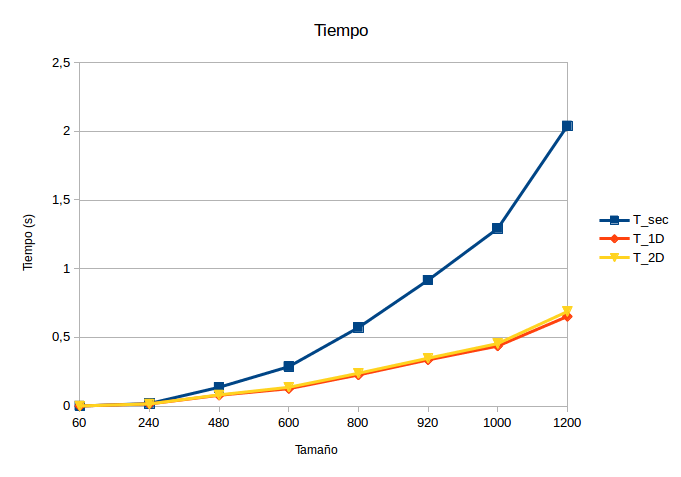
\includegraphics[width=9cm]{img/tiempo}
	\caption{Gráfica de tiempo para P = 4 y N = 64, 128, 256, 512 y 1024}
	\label{fig:grafica_tiempo}
\end{figure}

\begin{figure}[H]
	\centering
	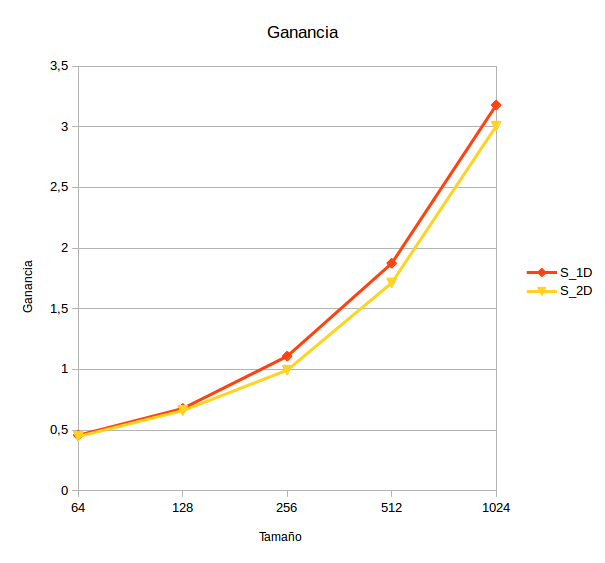
\includegraphics[width=9cm]{img/ganancia}
	\caption{Gráfica de ganancia para P = 4 y N = 64, 128, 256, 512 y 1024}
	\label{fig:grafica_ganancia}
\end{figure}

\end{document}